\chapter{基于卷积神经网络的目标识别研究}
\section{概述}
\section{在仿真数据上的研究}
首先从数学上对本节的问题进行描述。设第三章所得到的B扫数据为一系列尺寸为$w\times h$的二维矩阵
$\mathbf{A}_i(i = 1...N)$,其中$N$代表所生成
B扫的总数量,$w$表示每道回波的采样点数,$h$表示每个B扫中所包含的波形道数。
对于每一个B扫$\mathbf{A_i}$,还可以设$m_i$、$p_i$、$s_i$、$d_i$分别为其建模时设定的目标材质、
目标水平位置、目标尺寸和目标深度。目标材质$m_i$为取值范围是0到3的整数,分别代表“无目标”、“岩石”,
“水”,“金属”这几种情况。本节的目的就是设计并训练深度神经网络使其对于给定的$\mathbf{A_i}$可以
较为近似地输出$m_i$、$p_i$、$s_i$、$d_i$的预测值$m_i^{\prime}$、$p_i^{\prime}$、$s_i^{\prime}$、
$d_i^{\prime}$。

就如何预测这四个值的问题,笔者做如下考虑。目标材质$m_i$是一个只有四种取值的离散值,所以对于材质
的预测是一个典型的分类问题,可以尝试用多层卷积网络辅之以softmax分类器解决。而$p_i$、$s_i$和$d_i$
的取值都是一个连续的实数,不能按常见的多分类问题处理。对于水平位置$p_i$和尺寸$s_i$,
可以联系到探地雷达数据的以下两个特点:第一,只有收发天线移动到目标附近时才会产生明显的反射信号;
第二,目标的尺寸将影响到B扫图像上反射信号的持续范围。基于这两个特点,可以设想若对于天线移动过程中的
所有位置均作材质预测,而不是对于整幅B扫图像作单一的预测,则可以利用材质预测的结果对目标水平位置和
尺寸做出判断。而对于深度值$d_i$,笔者拟采用处理回归问题的方法输出连续的预测值。
\subsection{数据预处理}
在设计和训练深度网络之前,首先必须准备好训练样本$\mathbf{X}_{train}$、训练样本标签$\mathbf{Y}_{train}$、
测试样本$\mathbf{X}_{test}$、测试样本标签$\mathbf{Y}_{test}$。由于在这里要对天线经过的每个位置均
做出材质预测,所以必然要对原始B扫数据做出切分处理,使得天线经过的每个位置都对应一小块B扫图像的子区域,
另外还需要在样本标签中设置对应这些子区域的标签向量来表示实际的材质。完整的数据切分过程如下:

1. 定义图像子区域的尺寸为$w_{sub}\times h$,天线每次移动距离为$d_{antenna}$,其中$w_{sub}$为子区域的宽度,其值大致等于B扫图像中双曲线
图案宽度的一半。

2. 设训练样本由$\mathbf{A}_1$...$\mathbf{A}_{N^{\prime}}$产生,
训练样本由$\mathbf{A}_{N^{\prime} + 1}$...$\mathbf{A}_{N}$产生,
则训练和测试样本按如下公式产生:
\begin{equation}
	\begin{aligned}
	\mathbf{X_{train}}[k] &= \mathbf{A}_i[x_{start}:x_{start} + w_{sub}]\qquad (i = 1...N^{\prime})\\
	\mathbf{X_{test}}[k] &= \mathbf{A}_i[x_{start}:x_{start} + w_{sub}]\qquad (i = N^{\prime} + 1...N)
	\end{aligned}
\end{equation}
其中$i = 1...N$,$x_{start} = 1...w - w_{sub}$,$k = 1 ... i \times (w-w_{sub})$;符号$A[a:b]$代表从$a$行
到$b$取子矩阵。

3. 训练样本标签和测试样本标签由收发天线中心到目标物水平位置的距离是否小于目标尺寸的两倍确定,写成公式形式为:
$$
\mathbf{Y}[i] = 
	\begin{cases} 
		onehot(m_i) & |(x_{start} + w_{sub} / 2 - \frac{p_i}{d_{antenna}}| \leq \frac{2 s_i}{d_{antenna}} \\
		onehot(1)   & Others
	\end{cases}
$$
其中$onehot(m_i)$函数表示将介质类型所对应的整数转化为对应的四阶向量形式,即$onehot(1)=[1\quad 0 \quad 0 \quad 0]$,
$onehot(2)=[0\quad 1 \quad 0 \quad 0]$...$onehot(4)=[0\quad 0 \quad 0 \quad 1]$。
\begin{figure}[htbp]
	\includegraphics{bscan_slice.pdf}
	\caption[]{B扫数据切分示意图}
	\label{bscan_slice}
\end{figure}

图\ref{bscan_slice}为数据切分过程的示意图。图中的B扫图像对应的是某金属目标的图像,所以在目标附近的子图像对应的
标签为[0 0 0 1],而远离目标的子图像对应的标签为[1 0 0 0],表示无目标。

接下来还需要对样本数据进行更进一步的处理,分别是时间子采样和归一化。进行时间子采样的原因是雷达B扫数据特别是仿真得出
的B扫数据往往在时间方向上的数据点数$w$比行进距离方向的数据点数$h$多一个量级以上,这样既会导致数据量太大影响
训练速率也会导致切分后的子图像的纵横比过大而导致矩形卷积核无法图像上的目标特征,因此在不影响图像本来形态的情况下
可以对原始数据在时间方向上做子采样处理,使纵横比大致处于一个量级。而归一化操作的目的是使所有数据的值限定在[0, 1]范围
内,从而使所有的样本都处于同一量级,避免奇异样本的影响。

时间子采样处理的数学表达为:
\begin{equation}
	\mathbf{A}^{\prime}_i[m, n] = \mathbf{A}_i[m, t_{sample} n] \qquad
	 (i = 1...N, m = 1...h, n = 1...[\frac{w}{t_{sample}}]) 
\end{equation}

常见归一化方法为最大最小归一化,其数学表达式为:
\begin{equation}
	\mathbf{X}_i^{\prime}=\frac{\mathbf{X}_i-\min (\mathbf{X}_i)}
	{\max (\mathbf{X}_i)-\min (\mathbf{X}_i)}
\end{equation}

经过前面的处理,第三章的100幅B扫数据被处理为17820道数据,其中各类型的样本数量如表\ref{table_sample_kind_unbalanced}所示。
\begin{table}[h]
	\caption{各类型样本数量} 
	\begin{tabular}{|c|c|c|} 
		\hline  
		样本类型 &  数量\\
		\hline 
		无目标 & 13385 \\  
		\hline  
		岩石 & 1507 \\  
		\hline  
		水 & 1142\\
		\hline
		金属 & 1386 \\
		\hline  
	\end{tabular}
	\label{table_sample_kind_unbalanced}
\end{table}

可以看出四种类型的样本中,岩石、水和金属的样本数量大致相等而无目标样本的数量远远大于其他类型,这样会导致
样本不平行的问题,从而影响后面深度神经网络的训练结果。为了解决这个问题可以在无目标样本中剔除部分数据,
使其剩余数量等于其他三类样本数量的平均值。

\subsection{网络结构设计与训练}
本节所设计的网络结构以图\ref{cnn_structure}所示的卷积神经网络为基础,而具体的各层参数经过不断地试验尝试,
得到反复改进,最终形成了如表\ref{table_network_structure}所示的网络结构。
\begin{table}[h]
	\caption{地下目标识别神经网络结构} 
	\begin{tabular}{|c|c|c|} 
		\hline  
		层数 &  类型 & 参数\\
		\hline 
		1 & 卷积层 & 32个$3\times 5$的核;relu激活\\  
		\hline  
		2 & Dropout层 & 丢弃率:0.25\\
		\hline
		3 & 汇聚层 & $2\times 2$最大汇聚\\
		\hline
		4 & 卷积层 & 64个$3\times 5$的核;relu激活\\  
		\hline  
		5 & Dropout层 & 丢弃率:0.25\\
		\hline
		6 & 汇聚层 & $2\times 2$最大汇聚\\
		\hline
		7 & 卷积层 & 128个$3\times 5$的核;relu激活\\
		\hline  
		8 & Dropout层 & 丢弃率:0.25\\
		\hline
		9 & 卷积层 & 128个$3\times 5$的核;relu激活\\
		\hline  
		10 & Dropout层 & 丢弃率:0.25\\
		\hline
		11 & 卷积层 & 128个$3\times 5$的核;relu激活\\
		\hline  
		12 & Dropout层 & 丢弃率:0.25\\
		\hline
		13 & 卷积层 & 128个$3\times 5$的核;relu激活\\
		\hline  
		14 & Dropout层 & 丢弃率:0.25\\
		\hline
		15 & 全连接层 & 神经元数量:4;激活函数:softmax\\
		\hline  
	\end{tabular}
	\label{table_network_structure}
\end{table}

Dropout: A Simple Way to Prevent Neural Networks from Overfitting。
此网络共使用了6层卷积结构,在每个卷积网络层之后均使用了Dropout层。Dropout层的作用是缓解深度神经网络常出现
的过拟合问题。所谓过拟合,就是指在有限的数据上拟合了过于复杂的模型,从而使模型学习了数据上过于细节的特征。
过拟合会使模型在新数据上的泛化能力不够。将多个模型组合起来也能被用来减轻过拟合的问题,但是这种方法需要
消耗很多的模型训练时间。Dropout层在减轻过拟合方面不需要额外的计算消耗而且效果明显,其基本思路是在训练过程中
随机选择一些神经元并将它们以及它们与前后层之间的连接从网络中暂时删除,其作用相当于在训练过程中引入噪声和稀疏性
并迫使网络学习到数据中更加高阶的结构。

模型中各卷积层的尺寸设置为$3\times 5$,这是因为输入数据的形状基本呈竖长条状($50\times 128$),为了更好地匹配
输入数据的维度,这里在保持卷积核较小的情况下应该尽量使其宽高比接近于输入数据的宽高比。

另外每个卷积层的卷积核数量,即特征图的数量,在使用汇聚层之后均成倍增加。比如从第四层到第七层卷积核数就从64
增加到了128。这样做的考虑是汇聚层的使用会使数据
丢失近一半的信息(图像的尺寸减半),所以应增加特征图数量来弥补这一问题。
\begin{figure}[htbp]
	\includegraphics{loss_curve.pdf}
	\caption[]{损失函数曲线}
	\label{loss_curve}
\end{figure}
\begin{figure}[htbp]
	\includegraphics{acc_curve.pdf}
	\caption[]{训练正确率曲线}
	\label{acc_curve}
\end{figure}
\subsection{结果分析}
为了直观地展示上节神经网络的预测结果,图\ref{material_prediction}给出了某幅测试样本中的B扫在
相同的横坐标下目标介质识别问题的预测结果和实际结果,底部的B扫图像可作为预测结果的参照。
\begin{figure}[htbp]
	\includegraphics{material_prediction_80.pdf}
	\caption[]{预测结果与B扫对比图}
	\label{material_prediction}
\end{figure}

可以看出对于该测试B扫,预测曲线和实际曲线高度吻合,目标的性质岩石识别正确,仅在目标左侧预测曲线的范围略微
超出实际曲线的范围。按照4.2.1节的讨论,其中所使用的图像切分使得预测结果与天线位置信息相关,
实际曲线中位于目标位置上方的矩形窗的宽度也与目标的尺寸相关。所以利用介质类别的预测结果曲线,也可以间接
对目标的水平位置和尺寸做出预测。

设某幅B扫图像$\mathbf{A}_i$预测曲线为取值为0到4的一维整数数组$\mathbf{P}$,其值分别对应无目标、岩石、水和金属这几种
情况。对于整幅B扫图像,介质种类的预测结果$m_i^{\prime}$可由$\mathbf{P}$中的最大值$max(\mathbf{P})$来表示。而
介质的水平位置可用矩形窗的中心来计算,即:
\begin{equation}
	p_i^{\prime} = mean(nonzero(\mathbf{P}))\times d_{antenna}
\end{equation}
其中函数$nonzero$表示求解数组中非零元素的下标,函数$mean$用来求解平均数。

目标尺寸的预测结果$s_i^{\prime}$的计算方法为:
\begin{equation}
	s_i^{\prime} = \frac{1}{4 p_i^{\prime}}\sum{\mathbf{P}}\times d_{antenna}
\end{equation}

图\ref{material_bar}绘出了在测试B扫数据上目标材质$m_i$与$m_i^{\prime}$的详细对比结果,可以看到除了第13组所有
测试B扫均预测正确,综合正确率为95\%。
\begin{figure}[htbp]
	\includegraphics{material_bar.pdf}
	\caption[]{目标材质预测结果}
	\label{material_bar}
\end{figure}
\begin{figure}[htbp]
	\subfigure[]{
		\includegraphics{position_bar.pdf}}
	% \subfigure[]{
	% 	\includegraphics{position_error_bar.pdf}}
	\caption{目标水平位置预测结果}
	\label{position_bar}
\end{figure}
\begin{figure}[htbp]
	\subfigure[]{
		\includegraphics{size_bar.pdf}}
	% \subfigure[]{
	% 	\includegraphics{size_error_bar.pdf}}
	\caption{目标尺寸预测结果}
	\label{size_bar}
\end{figure}
\section{在实验数据上的研究}
为了验证前述深度网络在实测雷达B扫数据上的效果,本节采用某次在沙坑进行的探地雷达金属地雷目标探测实验的数据并尝试
对目标的所在位置进行识别。
\subsection{实验情况介绍}
现场实验使用自行开发的超宽带(UWB)GPR系统[cite]进行。该系统由发射器,天线,接收器,数据采集板和安装有控制软件的PC机组成。超宽带电磁脉冲通过第三章所述Vivaldi天线由双极性高斯脉冲源辐射,工作频率为210MHz,最大电压为830V。然后,反射信号由另一个天线接收并传送到数据采集板。信号在数据采集板中进行采样和数字化,并通过串口传输到pc软件。 2D扫描图像和其他系统指标在PC软件上实时显示。
\begin{figure}[htbp]
	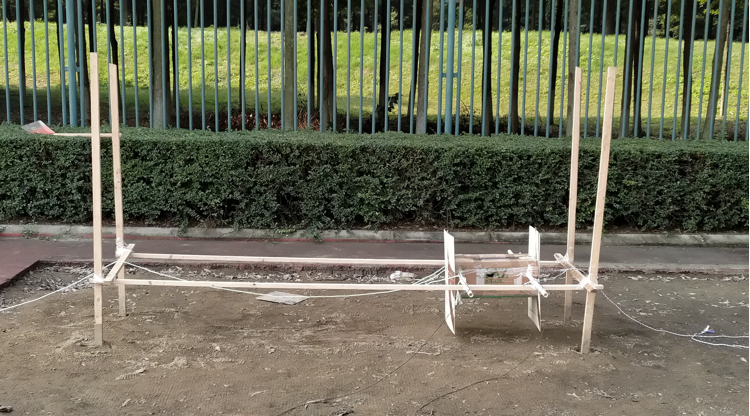
\includegraphics{sandpit_photo.png}
	\caption[]{沙坑实验现场}
	\label{sandpit_photo}
\end{figure}

实验场地位于电子科技大学清水河校区体育场的跳远沙坑中(图\ref{sandpit_photo})。该测试旨在检测非实验室环境中的地雷。实验在雨后两天进行,以确保土壤中适当的含水量。土壤含水量高会导致电磁波强烈衰减,因此难以成功探测到地雷。沙坑表面呈起伏状,大致起伏范围为-1.5cm到+1.5cm。
\begin{figure}[htbp]
	\includegraphics{sandpit_model.pdf}
	\caption[]{沙坑实验示意图}
	\label{sandpit_model}
\end{figure}

实验使用木架搭建了一个简易滑轨,滑轨长3米,收发天线被固定在纸箱两侧并可沿着水平木架行进。实验时,收发天线可由固定在两侧的绳子来回拉动。

由于没有实际的地雷,所以用某个$10\times 10$cm的铁板来代替。实验期间一共收集了7组雷达B扫数据。
第一组实验时沙坑内没有填埋任何物体。在进行第2组到第6组实验时,铁板分别填埋在图\ref{sandpit_model}中所标识的A-E处。第7组实验时,铁板放置在位置F处,并将塑料瓶埋入50厘米远的地方作为干扰物。1到6组数据用作训练样本。跟踪组7是测试数据。进行每组实验时,天线都会在木架上被来回拉动20次,所以实验共取得140道雷达B扫数据。
\subsection{数据预处理}
本章前面小节建立的数据切分方案完全可以直接用到实测数据的处理上,所以具体的预处理过程不再赘述。在这里只需要注意几个问题:

1. 本次实验中由于不涉及分类问题,所以在这里标签不再是长度为4的向量,而是长度为2的向量,且可能的取值为
[1 0]或者[0 1],分别用来代表当前位置有目标和当前位置没有目标。

2. 本次实验标签无法通过计算机程序直接计算得出,而是需要根据现场的实验记录人工标注。

通过切分处理,最后共得到7266组训练样本和1038组测试样本。
\subsection{网络训练和结果分析}
\begin{figure}[htbp]
	\includegraphics{sandpit_result.pdf}
	\caption[]{沙坑实验结果示例}
	\label{sandpit_result}
\end{figure}

\begin{table}[h]
	\caption{各类型样本数量} 
	\begin{tabular}{|c|c|c|} 
		\hline  
		正确率 & 虚警率 & 漏报率\\
		\hline
		94.2\% & 3.9\% & 1.9\%\\
		\hline
	\end{tabular}
	\label{table_sanpit_acc}
\end{table}
\section{本章小结}
